\subsection{Gekoppelte Pendel}
Durch Ermittlung der Schwingungsfrequenz der Phase und der Gegenphase, kann mithilfe von Gleichung \ref{eq:schwebung} die Schwebungsfrequenz berechnet werden. Die Messwerte sowie die Berechnungen sind in Tabelle \ref{tb:values} dargestellt.
Exemplarisch werden die gleichphasigen Schwingungen (Abbildung \ref{fig:gleich1}), die gegenphasigen Schwingungen (Abbildung \ref{fig:gegen1}) und die Schwebung (Abbildung \ref{fig:schwebung1}) inklusive der zugehörigen Fits von der zweiten Feder in Loch eins abgebildet. Bei diesem Aufbau ist vor allem die Schwebung sehr gut zu erkennen, weswegen dieser Aufbau gewählt wurde. Da der Ausschlag der beiden Pendel in y-Richtung durch das Messgerät verschoben wurde, wird jeweils die Theoriekurve des zweiten Pendels dargestellt.

\begin{figure}
\begin{center}
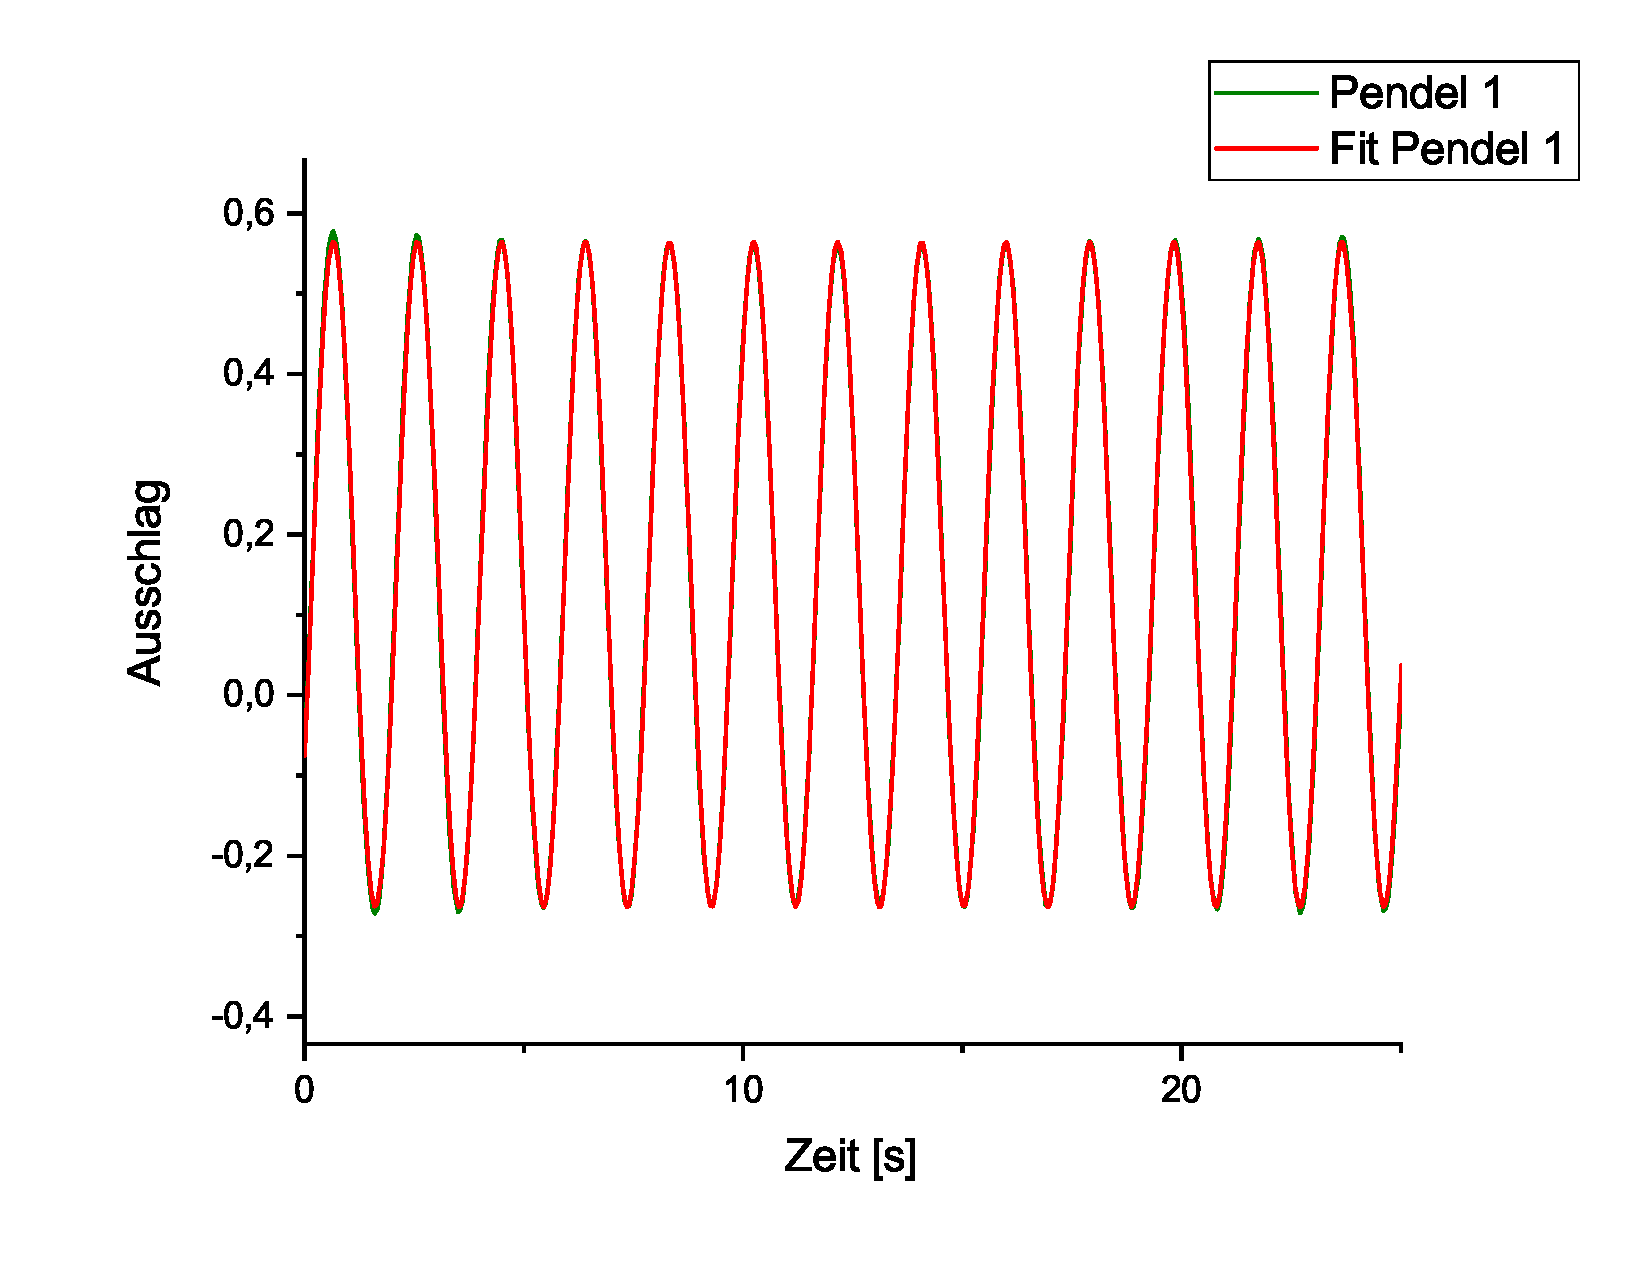
\includegraphics[width=0.8\textwidth]{Bilder/Feder2_gleich.eps}
\caption{Gleichphasige Schwingung der zweiten Feder in Loch 1 eingehängt.}
\label{fig:gleich1}
\end{center}
\end{figure}

\begin{figure}
\begin{center}
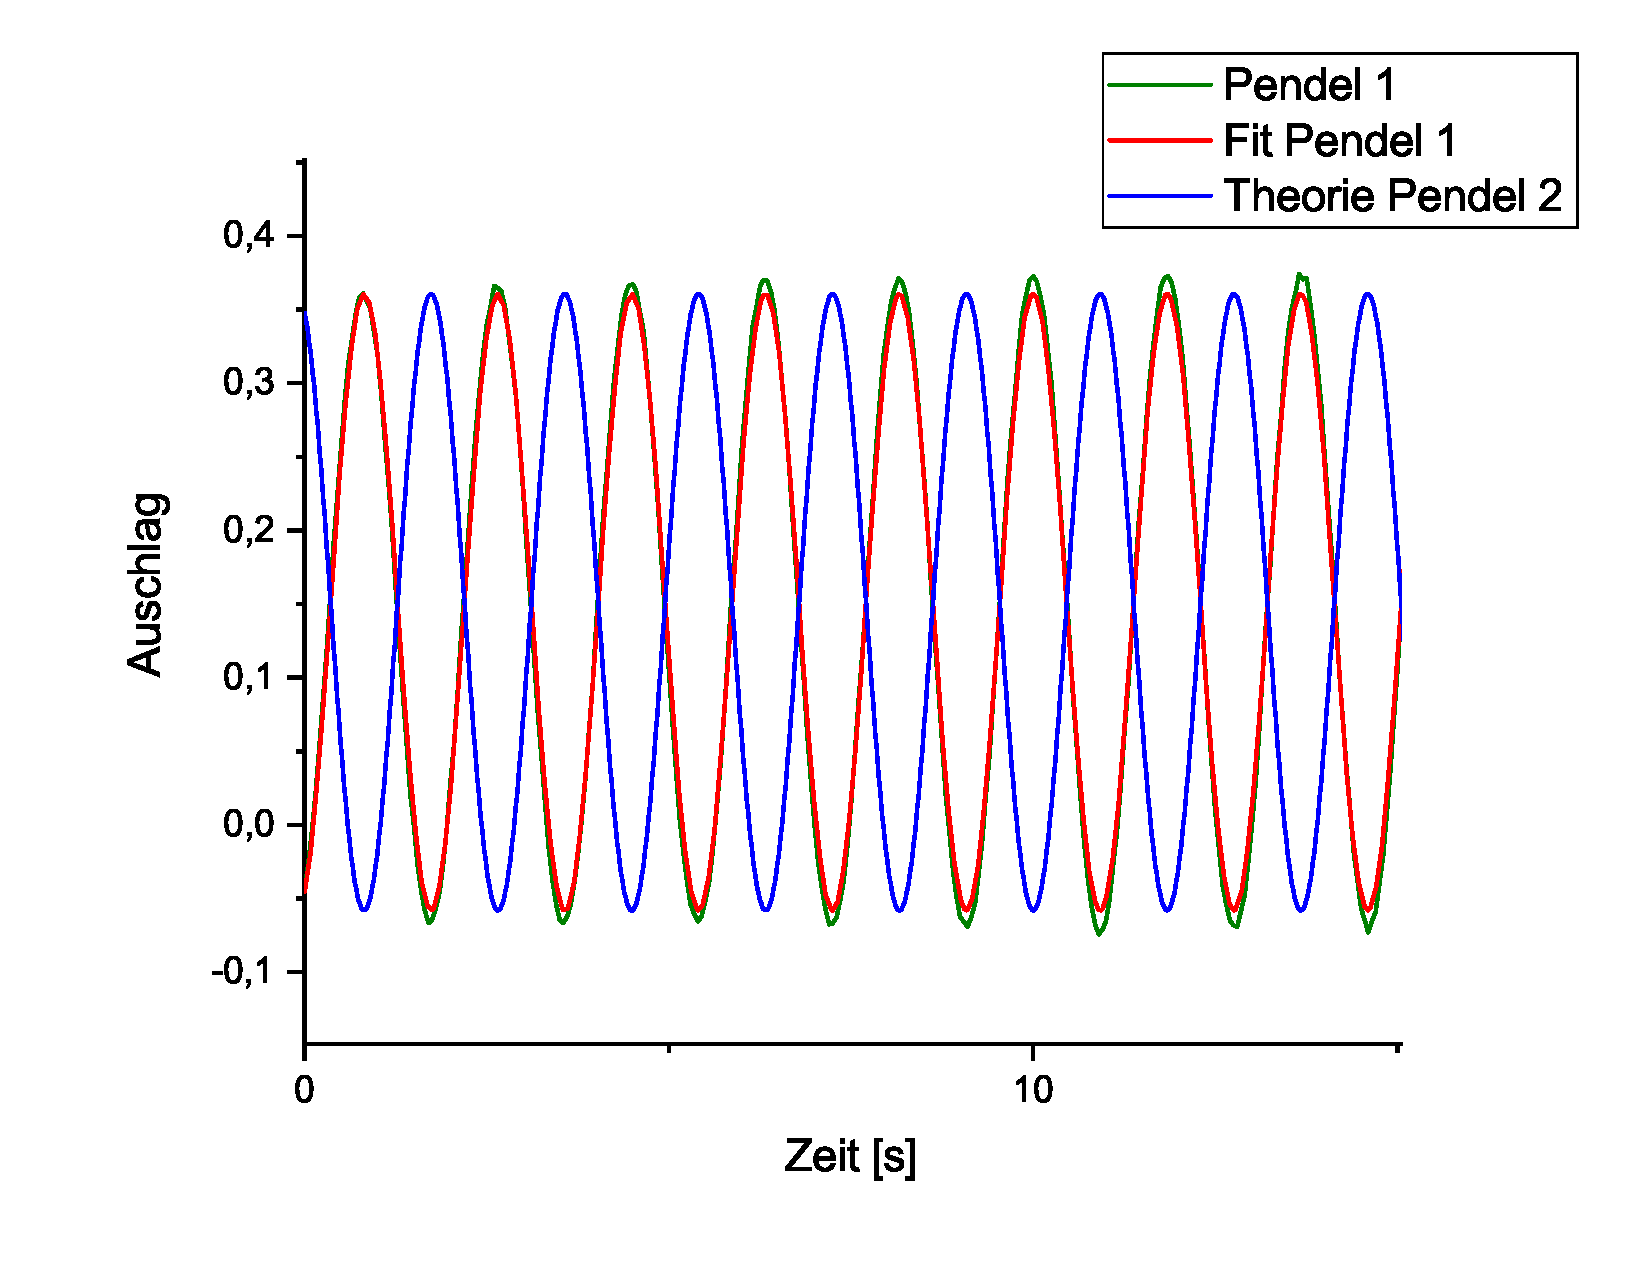
\includegraphics[width=0.8\textwidth]{Bilder/Feder2_gegen.eps}
\caption{Gegenphasige Schwingung der zweiten Feder in Loch 1 eingehängt.}
\label{fig:gegen1}
\end{center}
\end{figure}

\begin{figure}
\begin{center}
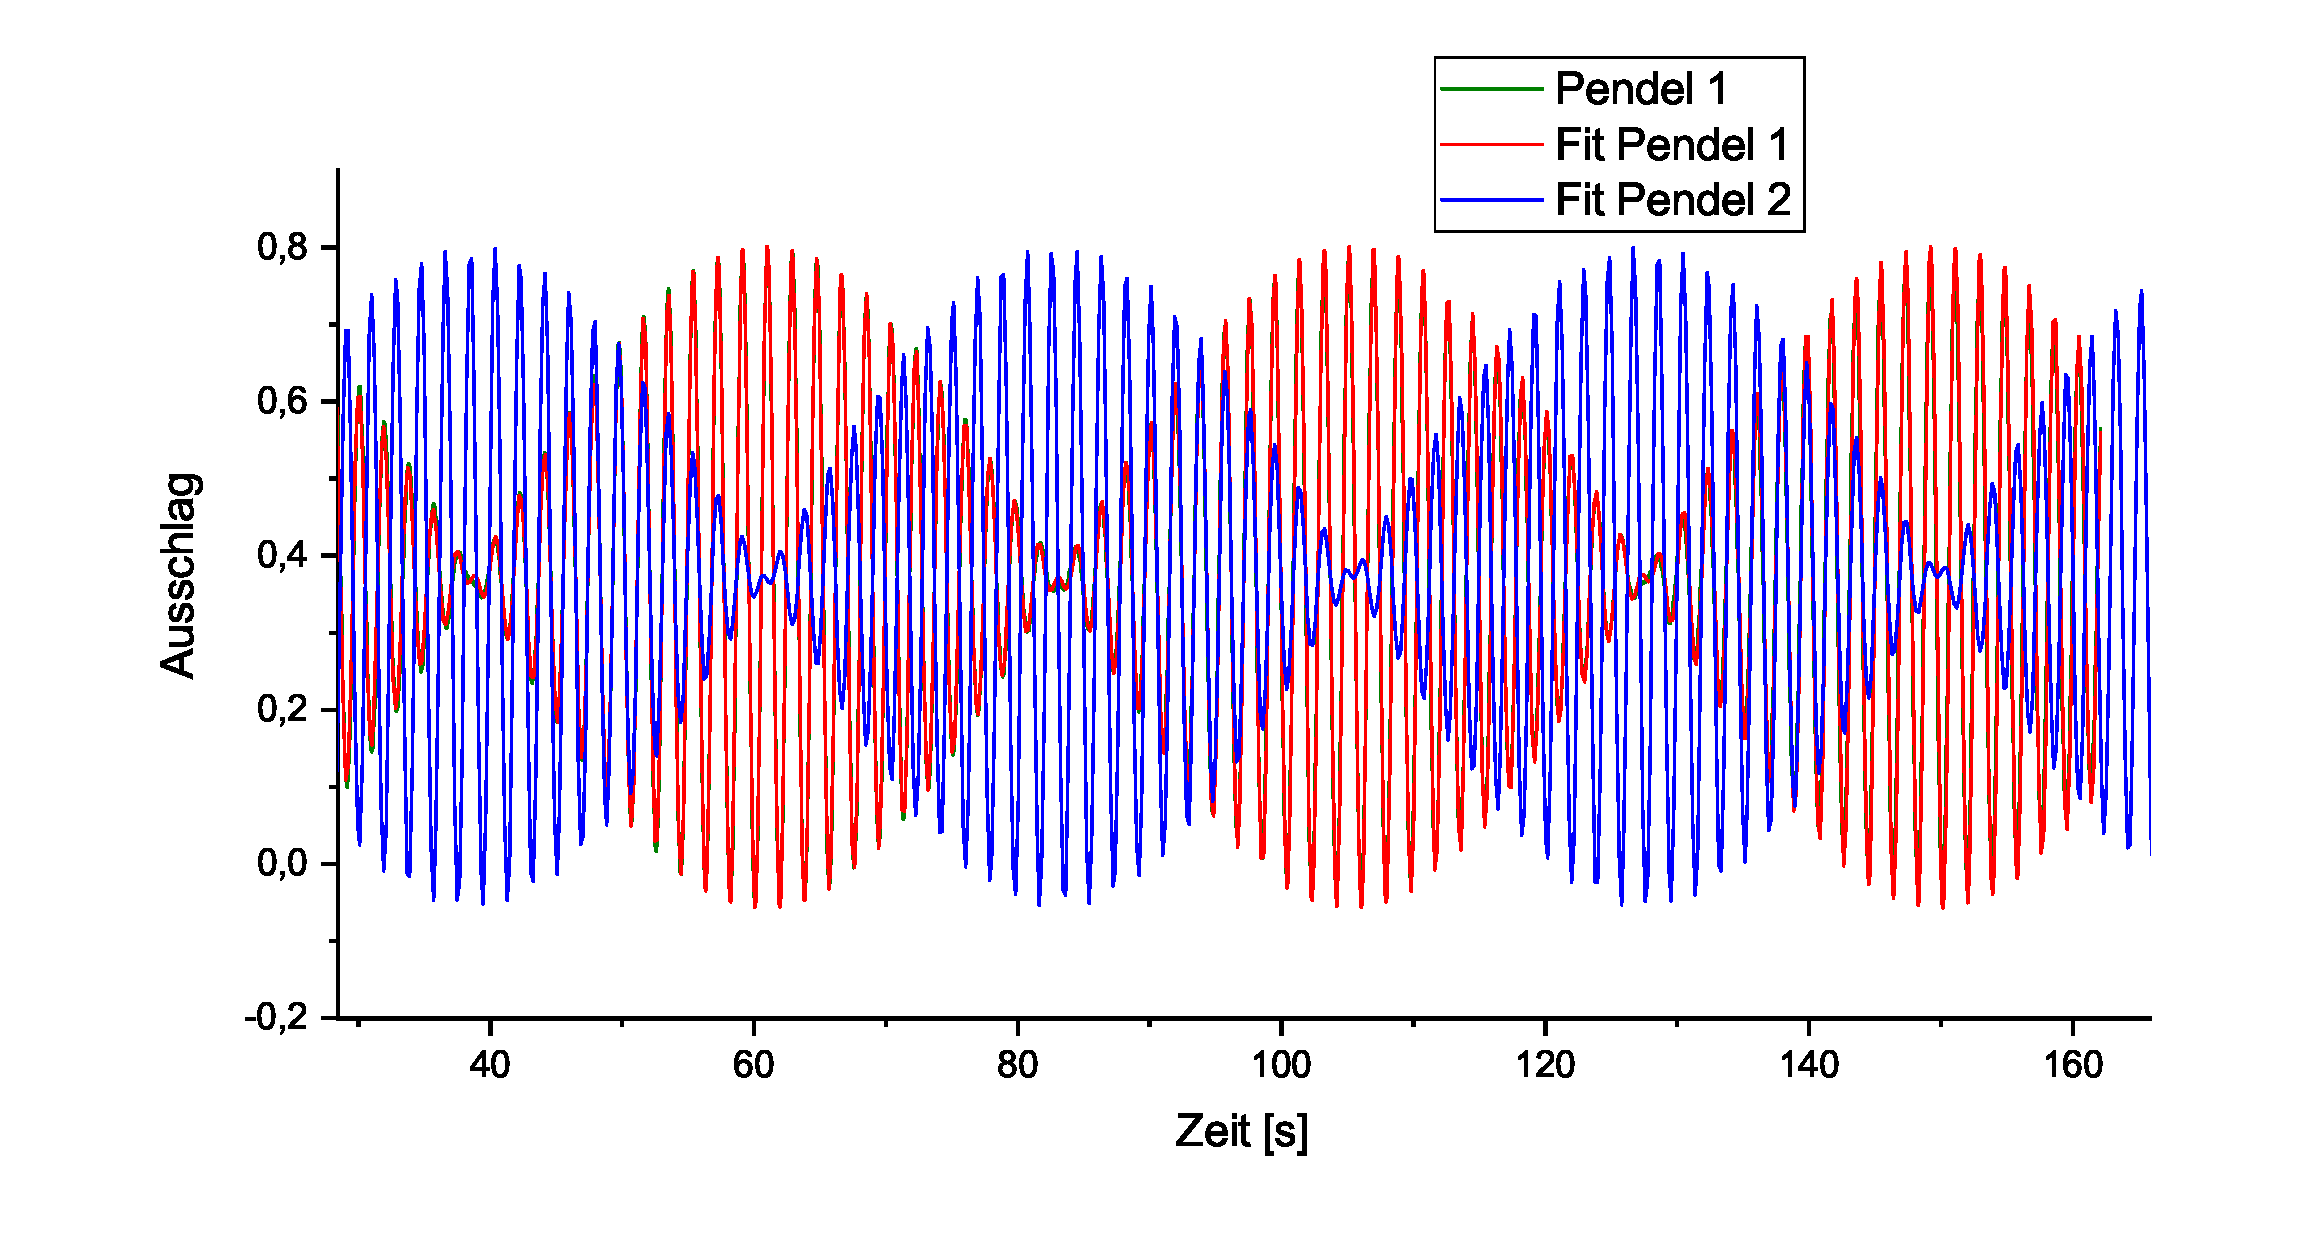
\includegraphics[width=0.8\textwidth]{Bilder/Feder2_Schwebung.eps}
\caption{Schwebung der zweiten Feder in Loch 1 eingehängt.}
\label{fig:schwebung1}
\end{center}
\end{figure}



\begin{table}
\resizebox{\linewidth}{!}{
% \begin{tabular}{|c|c|c|c|c|c|}
% \hline 
% • & 28.2 mm & 53.2 mm & 78.2 mm & 102.2 mm & 28.2 mm / Feder 2 \\ 
% \hline 
% $T_\mathrm{gl}/2$ & $\unit[(0.95841 \pm 1.1\e{-5})]{s}$ & $\unit[(0.95798 \pm 1.3\e{-5})]{s}$ & $\unit[(0.95724 \pm 3.2\e{-5})]{s}$ & $\unit[(0.95781 \pm 1.1\e{-5})]{s}$ & $\unit[(0.95826 \pm 1.3\e{-5})]{s}$ \\ 
% \hline 
% $T_\mathrm{geg}/2$ & $\unit[(0.92861 \pm 1.8\e{-5})]{s}$ & $\unit[(0.86739 \pm 1.1\e{-5})]{s}$ & $\unit[(0.79031 \pm 1.1\e{-5})]{s}$ & $\unit[(0.71542 \pm 1.1\e{-5})]{s}$ & $\unit[(0.91844 \pm 2.0\e{-5})]{s}$ \\ 
% \hline 
% $\omega_\n{S}$ berechnet & $\unit[(0.0526 \pm 0.0044)]{s^{-1}}$ & $\unit[(0.1712 \pm 0.0044)]{s^{-1}}$ & $\unit[(0.3466 \pm 0.0044)]{s^{-1}}$ & 
% $\unit[(0.5556 \pm 0.0044)]{s^{-1}}$ & $\unit[(0.0711 \pm 0.0044)]{s^{-1}}$ \\ 
% \hline 
% $\omega_\n{S}$ experimentell & $\unit[(0.0519 \pm 0.0044)]{s^{-1}}$ & $\unit[(0.1708 \pm 0.0044)]{s^{-1}}$ & $\unit[(0.346988 \pm 16\e{-6})]{s}$ & val7 & 
% $\unit[(0.0706\pm0.0044)]{s^{-1}}$ \\ 
% \hline 
%\end{tabular} 
\def\arraystretch{1.2}
\begin{tabular}{c ccccccc}
    Feder & $r$ in $\unit{cm}$ & $T_\mathrm{gl}/2$ & $T_\mathrm{geg}/2$ & $\omega_\n{S}$ berechnet & $\omega_\n{S}$ exp. & $\omega_\n{M}$ berechnet & $\omega_\n{M}$ exp.\\[1mm]
    \hline
    1 & 28.2 & $0.958410(11)$ & $0.928610(18)$ & $0.053(3)$ & $0.052(3)$ & $3.331(5)$ & $3.325(3)$\\
    \hline
    1 & 53.2 & $0.957980(13)$ & $0.867390(11)$ & $0.171(3)$ & $0.171(3)$ & $3.451(5)$ & $3.451(3)$\\
    \hline
    1 & 78.2 & $0.95724(3)$ & $0.790310(11)$ & $0.347(3)$ & $0.347(3)$ & $3.629(5)$ & $3.628(3)$\\
     \hline
    1 & 102.2 & $0.957810(11)$ & $0.715420(11)$ & $0.556(3)$ & $0.556(3)$ & $3.836(5)$ & $3.836(3)$\\
    \hline
    2 & 28.2 & $0.958260(13)$  & $0.918440(20)$  & $0.071(3)$  & $0.071(3)$ & $3.350(5)$ & $3.348(3)$\\
    \hline
\end{tabular}
}
\caption{Angegeben wird der Abstand der $r$ Feder zum Aufhängepunkt und die halbe Schwingungsdauer der Gleich-/Gegenschwingungen bzw. die daraus berechneten und experimentell bestimmten einhüllenden Frequenzen $\omega_\n{S}$. Die Fehler bei $T_\mathrm{gl}/2$ und $T_\mathrm{geg}/2$ sind rein statistisch, bei $\omega_\mathrm{S}$ wurde der systematische Fehler berücksichtigt. Zeiten sind in Sekunden, Frequenzen in $\unit{s^{-1}}$ angegeben.}
\label{tb:values}
\end{table}

Die angegebenen Fehler beziehen sich auf die Regression. Allerdings weichen die Werte für die Schwingungen in Phase, die in der Theorie gleich sind, da die Feder nicht aus ihrer Gleichgewichtslage bewegt wird. Mithilfe dieser Werte können wir unseren systematischen Fehler auf etwa $\unit[0.001]{s}$ abschätzen. Für Kreisfrequenzen ergibt sich somit ein Fehler von ca. $\unit[0.0031]{s^{-1}}$. Die Berechnung des gesamten Fehlers berechnen wir also durch:

\begin{equation*}
\Delta \omega_\n{S} = \sqrt{
\left(\frac{1}{2} \cdot \Delta\omega_\n{gl}\right)^2
+ 
\left(\frac{1}{2} \cdot \Delta\omega_\n{geg}\right)^2
+
\left(\frac12 \unit[0.0031]{s^{-1}} + \frac12 \unit[0.0031]{s^{-1}} \right)^2
}
\end{equation*}

Für die mittleren Kreisfrequenzen sind die Rechnungen und die Fehlerrechnung analog dazu.

Wie hier sehr schön gesehen werden kann, spielen die Fehler durch die Regression kaum eine Rolle. Die größte Fehlerursache sind Störfaktoren wie z.B. unterschiedlich starke Reibung (durch unterschiedlich große Auslenkung usw.) welche sich in unterschiedlichen Messungen ändern.

Der Kopplungsgrad lässt sich durch Formel \ref{eq:kopplung} berechnen. Der Fehler hierfür ergibt sich durch:

\begin{equation*}
\Delta K = \sqrt{
\left(\Delta \omega_\n{geg}\frac{\partial \omega_\n{geg}}{\partial K}\right)^2
+
\left(\Delta \omega_\n{gl}\frac{\partial \omega_\n{gl}}{\partial K}\right)^2
}
\end{equation*}

Die Werte die wir erhalten stehen in Tabelle \ref{tb:K}.

\begin{table}[t]
\resizebox{\linewidth}{!}{\begin{tabular}{c|ccccc}
 & Loch 1 & Loch 2 & Loch 3 & Loch 4 & Loch 1 (Feder 2) \\ 
\hline 
K & $\unit[(0.0316 \pm 0.0013)]{s^{-1}}$ & $\unit[(0.099 \pm 0.0013)]{s^{-1}}$ & $\unit[(0.1893 \pm 0.0012)]{s^{-1}}$ & $\unit[(0.2838 \pm 0.0011)]{s^{-1}}$ & $\unit[(0.0424 \pm 0.0013)]{s^{-1}}$ \\ 
\end{tabular}}
\caption{Die berechnetet Werte für den Kopplungsgrad $K$}
\label{tb:K}
\end{table}


% Aufgabe 13 -----------------------------------------------------------------------------


\begin{figure}[h]
    \begin{tikzpicture}
    \begin{axis}[
    height=1.0\plotheight, width=\plotwidth,
    xlabel={Kopplungsabstand $r$}, ylabel={$\omega_\mathrm{S}$ und $\omega_\mathrm{M}$ in $\unit{s^{-1}}$},
    only marks,
    xmin=.22, xmax=1.08,
    ymax=4.15, ymin=-0.25,
    legend entries={Messwerte für $\omega_\mathrm{S}$, Theoriekurve, Messwerte für $\omega_\mathrm{M}$, Theoriekurve},
    legend style={at={(0.98,0.51)}, anchor=east},
    y tick label style={
        /pgf/number format/.cd,
        fixed,
        fixed zerofill,
        precision=1,
        /tikz/.cd
    },
    x tick label style={
        /pgf/number format/.cd,
        fixed,
        fixed zerofill,
        precision=1,
        /tikz/.cd
    }
    ]
    \addplot+ [color=blue, mark=o] table [x=r, y=w_S, col sep=comma] {./Daten/aufgabe13.csv};
    \addplot[domain=0.25:1.05, color=blue, smooth, thick, mark size=0] {-0.5*3.2805 + 0.5*sqrt(3.2805^2 + 2.8214^2*(x + 0.01294)^2)};
    % 
    \addplot+ [color=red, mark=square] table [x=r, y=w_M, col sep=comma] {./Daten/aufgabe13.csv};
    \addplot[domain=0.25:1.05, color=red, smooth, thick, mark size=0] {0.5*3.2805 + 0.5*sqrt(3.2805^2 + 2.8211^2*(x + 0.01294)^2)};
    
    \end{axis}
    \end{tikzpicture}
    \caption{Die Schwebungsparameter $\omega_\mathrm{S}$ und $\omega_\mathrm{M}$ in Abhängigkeit des Kopplungsabstands $r$ und die entsprechende Theoriekurve. Der Fehler ist kleiner als die Datenpunkte}
    \label{diag:wassolldas}
\end{figure}


\begin{figure}[h]
    \begin{tikzpicture}
    \begin{axis}[
    height=0.9\plotheight, width=\plotwidth,
    xlabel={Kopplungsabstand $r$}, ylabel={Kopplungsgrad $K$},
    only marks,
    legend entries={Messwerte, Theoriekurve},
    legend pos=south east,
    %xmin=.23, xmax=1.07,
    %ymax=4.15, ymin=-0.25
    y tick label style={
        /pgf/number format/.cd,
        fixed,
        fixed zerofill,
        precision=2,
        /tikz/.cd
    },
    x tick label style={
        /pgf/number format/.cd,
        fixed,
        fixed zerofill,
        precision=1,
        /tikz/.cd
    }
    ]
    \addplot+ [color=blue, mark=o, error bars/.cd, y dir=both, y explicit] table [x=r, y=K, y error=err_K, col sep=comma] {./Daten/aufgabe13.csv};
    \addplot[domain=0.25:1.05, color=blue, smooth, thick, mark size=0] {(x + 0.01294)^2 / (2.7045 + (x + 0.01294)^2)};
    % 
    \end{axis}
    \end{tikzpicture}
    \caption{Die Schwebungsparameter $\omega_\mathrm{S}$ und $\omega_\mathrm{M}$ in Abhängigkeit des Kopplungsabstands $r$ und die entsprechende Theoriekurve. Der Fehler ist kleiner als die Datenpunkte}
    \label{diag:K}
\end{figure}

Diagramm~\ref{diag:wassolldas} Zeig die $r$-Abhängigkeit von $\omega_\mathrm{S}$ und $\omega_\mathrm{M}$ und Diagramm~\ref{diag:K} die des Kopplungsgrades $K$.

Wir erwarten gemäß der Theorie, das $\omega_\mathrm{gl}$ konstant ist und weiter der Zusammenhand ${\omega_\mathrm{geg}}^2 = {\omega_\mathrm{gl}}^2 + 2 \frac{d \cdot r^2}{J}$ gilt. Mit Gleichungen~\ref{eq:avg} und \ref{eq:schwebung} ergeben sich die entsprechenden Beziehungen für $\omega_\mathrm{S}$ und $\omega_\mathrm{M}$. Unsere Messwerte folgen einem solchen Zusammenhang ideal (siehe Theoriekurven in Diagramm~\ref{diag:wassolldas}) falls man $r$ durch $r + \unit[1.3]{cm}$ substituiert. Das liegt wahrscheinlich daran, dass bei den Messungen von $r$ systematisch um diese Länge falsch gemessen wurde%
\footnote{tatsächlich hatten wir vergessen diese Strecken zu messen und mussten die Werte von einer anderen Gruppe erhalten.}%
.
Auch die Werte von $K$ passen, nach Korrektur von $r$, perfekt in den theoretischen Zusammenhang aus Gleichung~\ref{eq:kopplung}.














